\documentclass[12pt,letterpaper]{article}
\usepackage{graphicx,textcomp}
\usepackage{natbib}
\usepackage{setspace}
\usepackage{fullpage}
\usepackage{color}
\usepackage[reqno]{amsmath}
\usepackage{amsthm}
\usepackage{fancyvrb}
\usepackage{amssymb,enumerate}
\usepackage[all]{xy}
\usepackage{endnotes}
\usepackage{lscape}
\newtheorem{com}{Comment}
\usepackage{float}
\usepackage{hyperref}
\newtheorem{lem} {Lemma}
\newtheorem{prop}{Proposition}
\newtheorem{thm}{Theorem}
\newtheorem{defn}{Definition}
\newtheorem{cor}{Corollary}
\newtheorem{obs}{Observation}
\usepackage[compact]{titlesec}
\usepackage{dcolumn}
\usepackage{tikz}
\usetikzlibrary{arrows}
\usepackage{multirow}
\usepackage{xcolor}
\newcolumntype{.}{D{.}{.}{-1}}
\newcolumntype{d}[1]{D{.}{.}{#1}}
\definecolor{light-gray}{gray}{0.65}
\usepackage{url}
\usepackage{listings}
\usepackage{color}

\definecolor{codegreen}{rgb}{0,0.6,0}
\definecolor{codegray}{rgb}{0.5,0.5,0.5}
\definecolor{codepurple}{rgb}{0.58,0,0.82}
\definecolor{backcolour}{rgb}{0.95,0.95,0.92}

\lstdefinestyle{mystyle}{
	backgroundcolor=\color{backcolour},   
	commentstyle=\color{codegreen},
	keywordstyle=\color{magenta},
	numberstyle=\tiny\color{codegray},
	stringstyle=\color{codepurple},
	basicstyle=\footnotesize,
	breakatwhitespace=false,         
	breaklines=true,                 
	captionpos=b,                    
	keepspaces=true,                 
	numbers=left,                    
	numbersep=5pt,                  
	showspaces=false,                
	showstringspaces=false,
	showtabs=false,                  
	tabsize=2
}
\lstset{style=mystyle}
\newcommand{\Sref}[1]{Section~\ref{#1}}
\newtheorem{hyp}{Hypothesis}

\title{Problem Set 3}
\date{Sein Kim}
\author{Applied Stats/Quant Methods 1}

\begin{document}
	\maketitle

\section*{Question 1}
\vspace{.25cm}
\noindent We are interested in knowing how the difference in campaign spending between incumbent and challenger affects the incumbent's vote share. 
	\begin{enumerate}
		\item Run a regression where the outcome variable is \texttt{voteshare} and the explanatory variable is \texttt{difflog}.	\vspace{0.3cm}
		
		\noindent\textbf{R Code:}
		\lstinputlisting[language=R, firstline=41, lastline=51]{PS03_SK.R} \vspace{0.3cm}
		
		\noindent
		The fitted model is 
		\[
		\widehat{\text{voteshare}} = \hat{\beta}_0 + \hat{\beta}_1 \,\texttt{difflog}.
		\]
		From the output, $\hat{\beta}_1 > 0$, indicating that a one–unit increase in the log spending difference (i.e., the incumbent spends relatively more) is associated with a higher vote share for the incumbent. 
		The regression summary reports $R^2 =$ (value) and $n =$ (value).  
		These values suggest that spending differences explain a meaningful portion of variation in vote share.
		
		\vspace{0.3cm}
		
		\newpage	
		
		\item Make a scatterplot of the two variables and add the regression line. \vspace{0.3cm} 
		
		\noindent  \textbf{R Code:}
		\lstinputlisting[language=R, firstline=54, lastline=58]{PS03_SK.R}
		\vspace{0.3cm}
		\noindent
		
		\begin{figure}[H]\centering
			\caption{\footnotesize Scatterplot of \texttt{voteshare} and \texttt{difflog} with fitted regression line.}
			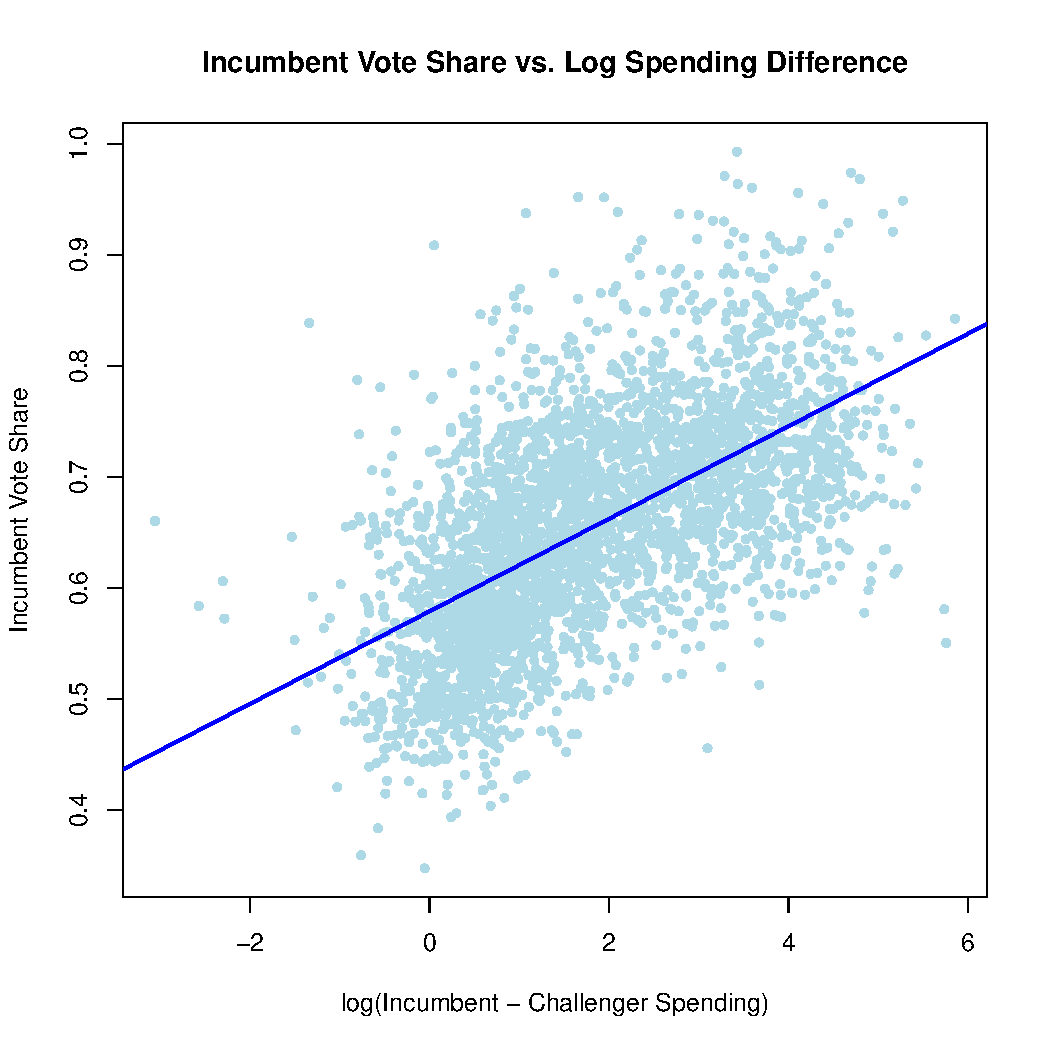
\includegraphics[width=0.7\textwidth]{q1_scatter.pdf}
		\end{figure}
		
		\noindent The scatterplot shows a clear positive linear trend, with the fitted regression line capturing the average upward slope: incumbents who spend relatively more tend to receive higher vote shares.
		
		\vspace{0.3cm}
	\newpage	
		\item Save the residuals of the model in a separate object.
		
		 \noindent\textbf{R Code (already executed above):}
		\lstinputlisting[language=R, firstline=41, lastline=42]{PS03_SK.R}
		
		\vspace{0.3cm}
		\noindent The residuals (\texttt{res\_q1}) capture the unexplained portion of the incumbent’s vote share after accounting for differences in campaign spending. 
		By saving these residuals, we isolate the variation in \texttt{voteshare} that is independent of \texttt{difflog}. 
		This residual variation will be used in Question 4 to examine whether the part of the vote share not explained by spending can instead be explained by presidential party support (\texttt{presvote})—an application of the Frisch–Waugh–Lovell theorem.
		
		\vspace{0.3cm}
		
		\item Write the prediction equation. \vspace{0.3cm}
		
		\noindent\textbf{Prediction Equation:}
		\[
		\widehat{\text{voteshare}} \;=\; \hat{\beta}_0 \;+\; \hat{\beta}_1\,\texttt{difflog}.
		\]
		Substituting the estimated coefficients from part (a) yields\\ 
		$\widehat{\text{voteshare}} = (\text{Intercept estimate}) + (\text{Slope estimate})\times\texttt{difflog}.$\\ 
		In addition, the script prints this equation to the console (via \texttt{b1 <- coef(m1)} and \texttt{cat(\ldots)} within lines 39–50), ensuring that the reported expression matches the fitted model exactly.
		
	\end{enumerate}
	
\newpage

\section*{Question 2}
\noindent We are interested in knowing how the difference between incumbent and challenger's spending and the vote share of the presidential candidate of the incumbent's party are related.	\vspace{.25cm}
	\begin{enumerate}
		\item Run a regression where the outcome variable is \texttt{presvote} and the explanatory variable is \texttt{difflog}.	
		 
		 \vspace{0.3cm}
		 \noindent\textbf{R Code:}
		\lstinputlisting[language=R, firstline=66, lastline=76]{PS03_SK.R}
		\vspace{0.3cm}
		\noindent
		The fitted model is 
		\[
		\widehat{\text{presvote}} = \hat{\beta}_0 + \hat{\beta}_1\,\texttt{difflog}.
		\]
		The regression output reports $R^2 =$ (value) and $n =$ (value).  
		The slope estimate $\hat{\beta}_1$ indicates whether districts with larger incumbent spending advantages tend also to be more favorable to the presidential party.
		
		\vspace{0.3cm}
		
		\item Make a scatterplot of the two variables and add the regression line. 
		
		\vspace{0.3cm}
		\noindent\textbf{R Code:}
		\lstinputlisting[language=R, firstline=79, lastline=86]{PS03_SK.R}
	\newpage	
		\noindent
		
		\begin{figure}[H]\centering
			\caption{\footnotesize Scatterplot of \texttt{presvote} and \texttt{difflog} with fitted regression line.}
			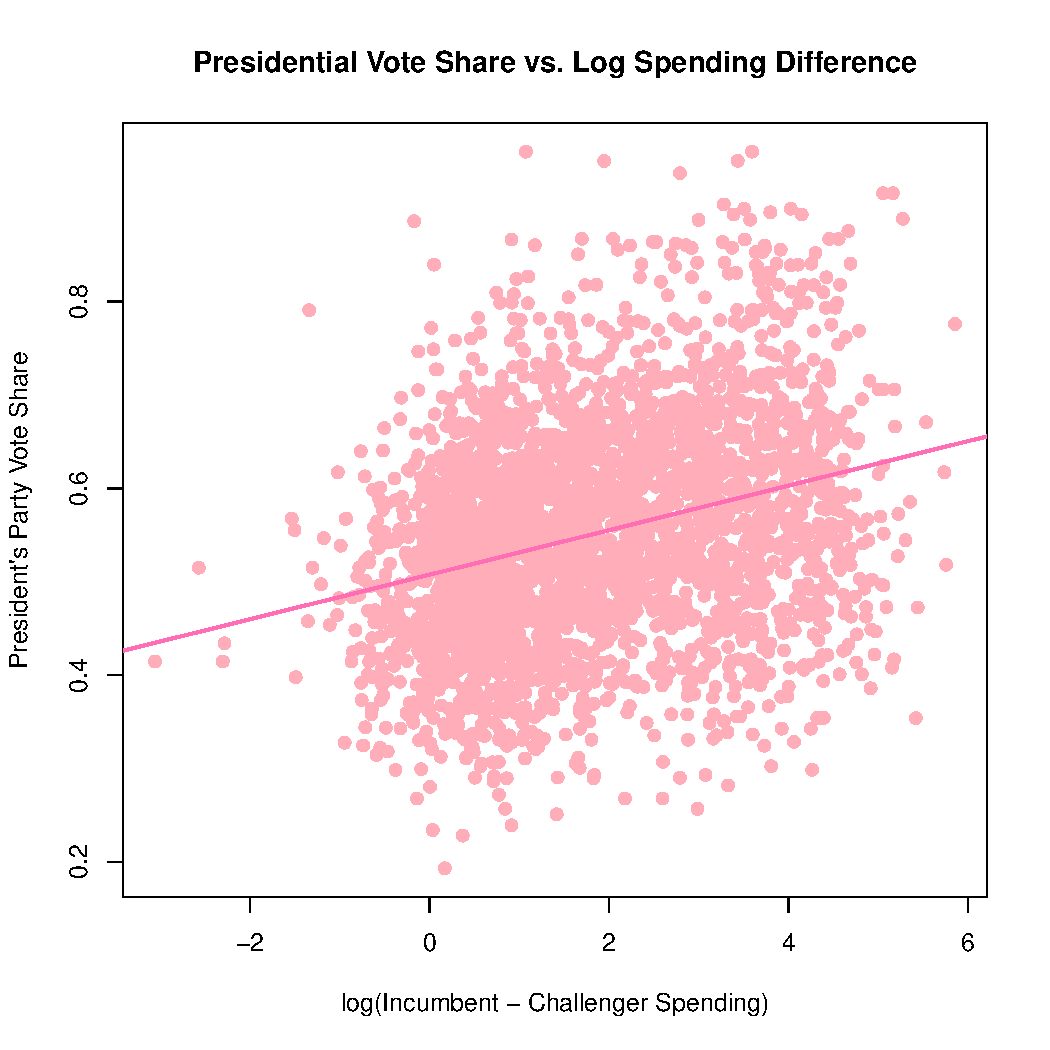
\includegraphics[width=0.7\textwidth]{q2_scatter.pdf}
		\end{figure}
		
		\noindent The plot shows the relationship between spending difference and presidential party vote share. The fitted line (abline(m2)) summarizes the average trend across districts, suggesting that areas with greater incumbent spending advantages tend to show slightly higher presidential vote shares.
		
		\vspace{0.3cm}
		
		\item Save the residuals of the model in a separate object. \vspace{0.3cm}
		
		 Residuals (\texttt{res\_q2}) capture the portion of \texttt{presvote} not explained by \texttt{difflog}. They will later be used in Question 4 to construct the added–variable regression.
		\vspace{0.3cm}
		
		\item Write the prediction equation. \vspace{0.3cm}
		The prediction equation is:
		\[
		\widehat{\text{presvote}} = \hat{\beta}_0 + \hat{\beta}_1\,\texttt{difflog}.
		\] 
		Substituting the estimated coefficients from part (a) gives the fitted linear model for the presidential party’s vote share.
		
		\end{enumerate}	
	
	\newpage	
\section*{Question 3}

\noindent We are interested in knowing how the vote share of the presidential candidate of the incumbent's party is associated with the incumbent's electoral success.
	\vspace{.25cm}
	\begin{enumerate}
		\item Run a regression where the outcome variable is \texttt{voteshare} and the explanatory variable is \texttt{presvote}. \vspace{0.3cm}
		
		\noindent\textbf{R Code:}
		\lstinputlisting[language=R, firstline=90, lastline=98]{PS03_SK.R} \vspace{0.3cm}
		
		\noindent
		The fitted model is 
		\[
		\widehat{\text{voteshare}} = \hat{\beta}_0 + \hat{\beta}_1\,\texttt{presvote}.
		\]
		A positive and statistically significant slope suggests that districts more favorable to the presidential party tend to yield higher vote shares for incumbents. 
		The regression summary reports $R^2 =$ (value), $\text{Adj. }R^2 =$ (value), and $n =$ (value).
		
		\vspace{0.3cm}
		
		\item Make a scatterplot of the two variables and add the regression line. \vspace{0.3cm}

		\noindent\textbf{R Code:}
		\lstinputlisting[language=R, firstline=101, lastline=108]{PS03_SK.R} \vspace{0.3cm}
		 		
		 \noindent
		\begin{figure}[H]\centering
			\caption{\footnotesize Scatterplot of \texttt{voteshare} and \texttt{presvote} with fitted regression line.}
			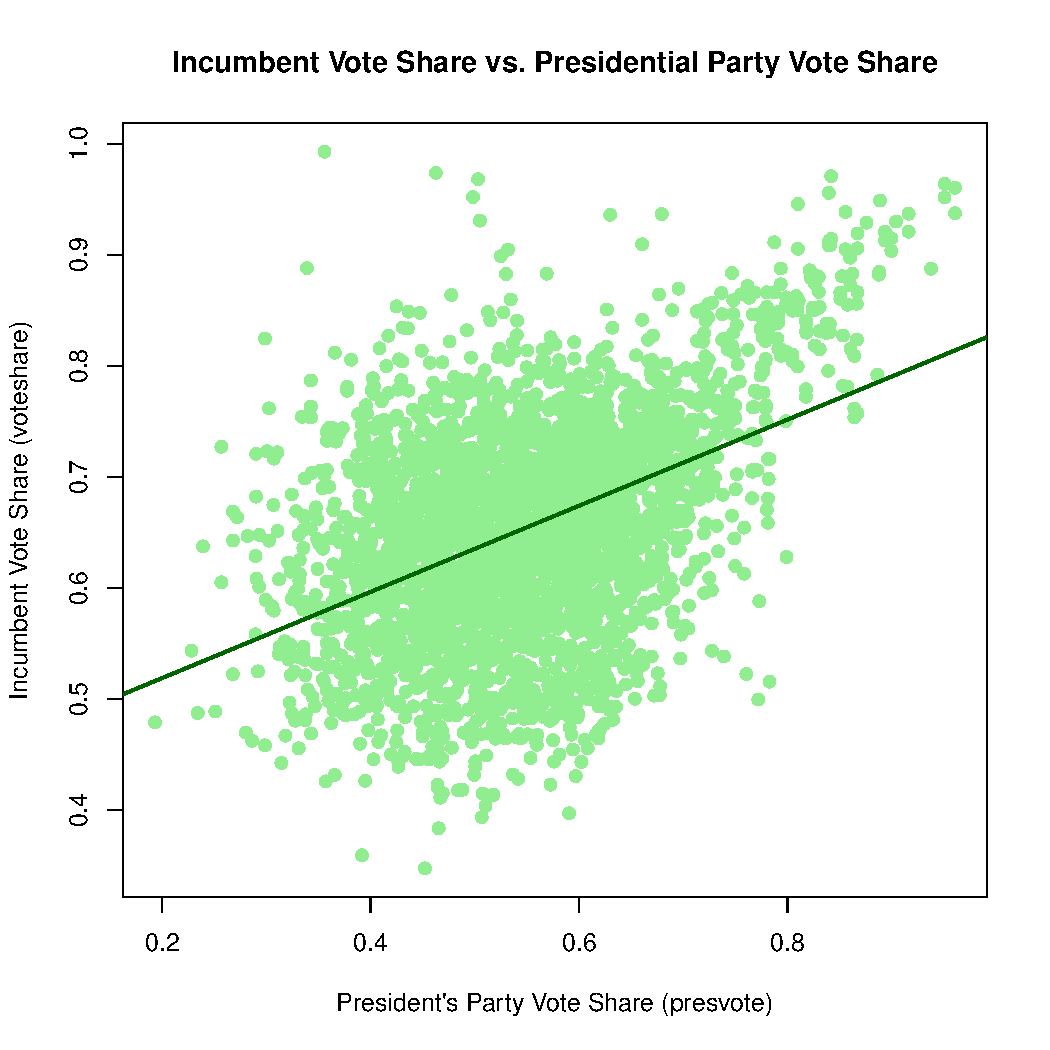
\includegraphics[width=0.7\textwidth]{q3_scatter.pdf}
		\end{figure}
		
		\noindent The plot shows a clear positive relationship between the presidential party’s vote share and the incumbent’s vote share.
		The fitted regression line (\texttt{abline(m3)}) indicates that incumbents tend to receive higher vote shares in districts where the president’s party performs strongly, suggesting that presidential popularity positively influences incumbents’ electoral success.
		
		\vspace{0.3cm}
		
		\item Write the prediction equation.
		
		 \vspace{0.3cm}
		  \noindent\textbf{Prediction Equation:}
		\[
		\widehat{\text{voteshare}} = \hat{\beta}_0 + \hat{\beta}_1\,\texttt{presvote}.
		\]
		Substituting the estimated coefficients from part (a) gives the fitted linear model for the incumbent’s vote share.
		
		
	\end{enumerate}
	

\newpage	
\section*{Question 4}
\noindent The residuals from part (a) tell us how much of the variation in \texttt{voteshare} is $not$ explained by the difference in spending between incumbent and challenger. The residuals in part (b) tell us how much of the variation in \texttt{presvote} is $not$ explained by the difference in spending between incumbent and challenger in the district.
	\begin{enumerate}
		\item Run a regression where the outcome variable is the residuals from Question 1 and the explanatory variable is the residuals from Question 2.
		\vspace{0.3cm}
		
		\noindent\textbf{R Code:}
		\lstinputlisting[language=R, firstline=112, lastline=120]{PS03_SK.R}
		\vspace{0.3cm}
		\noindent
		The fitted residual regression is 
		\[
		\widehat{\text{res\_q1}} \;=\; \hat{\alpha}_0 \;+\; \hat{\gamma}\,\texttt{res\_q2}.
		\]
		The estimate $\hat{\gamma}$ summarizes the linear association between the part of \texttt{voteshare} not explained by spending and the part of \texttt{presvote} not explained by spending. This added-variable regression shows that even after removing the effect of campaign spending, districts more favorable to the president’s party still give incumbents higher vote shares.
		
		\vspace{0.3cm}
		
		\item Make a scatterplot of the two residuals and add the regression line. 
		
		\vspace{0.3cm}
		\noindent\textbf{R Code:}
		\lstinputlisting[language=R, firstline=123, lastline=130]{PS03_SK.R}
		\vspace{0.3cm}
		
		\noindent
			
			\begin{figure}[H]\centering
				\caption{\footnotesize Added–variable plot: residuals from Q1 (\texttt{voteshare \textasciitilde{} difflog}) vs. residuals from Q2 (\texttt{presvote \textasciitilde{} difflog}).}
				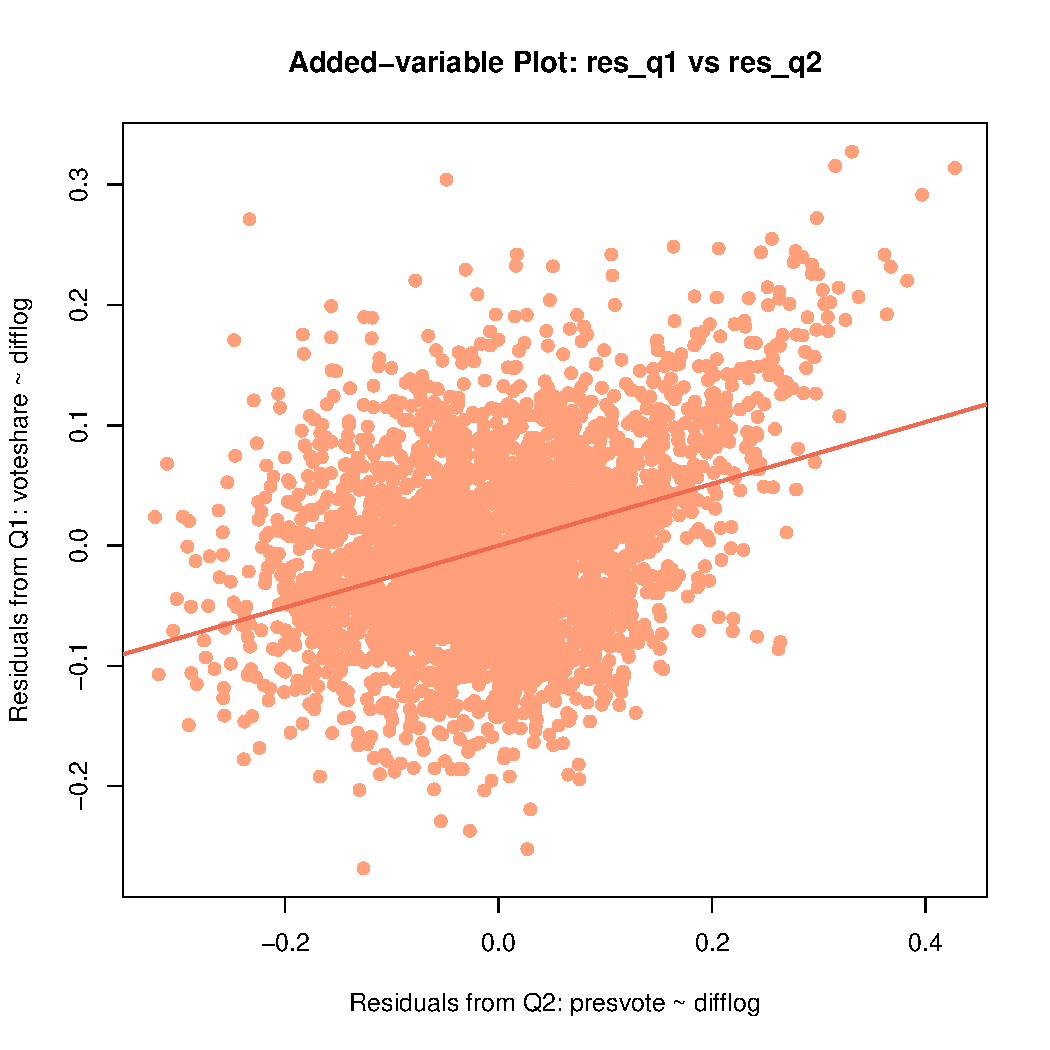
\includegraphics[width=0.7\textwidth]{q4_scatter.pdf}
			\end{figure}
			
			\vspace{0.3cm}
		
		\item Write the prediction equation.
		
		\vspace{0.3cm}
		\noindent\textbf{Prediction Equation:}
		\[
		\widehat{\text{res\_q1}} \;=\; \hat{\alpha}_0 \;+\; \hat{\gamma}\,\texttt{res\_q2}.
		\]
	\end{enumerate}
	
	\newpage	

\section*{Question 5}
\noindent What if the incumbent's vote share is affected by both the president's popularity and the difference in spending between incumbent and challenger? 
	\begin{enumerate}
		\item Run a regression where the outcome variable is the incumbent's \texttt{voteshare} and the explanatory variables are \texttt{difflog} and \texttt{presvote}.
		
		\vspace{0.3cm}
		\noindent\textbf{R Code:}
		\lstinputlisting[language=R, firstline=134, lastline=149]{PS03_SK.R}
		\vspace{0.3cm}
		\noindent\textbf
		The fitted model is
		\[
		\widehat{\text{voteshare}} = \hat{\beta}_0 + \hat{\beta}_1\,\texttt{difflog} + \hat{\beta}_2\,\texttt{presvote}.
		\]
		Here, $\hat{\beta}_1$ measures the spending effect \emph{controlling for} the political environment, and $\hat{\beta}_2$ measures the political environment effect \emph{controlling for} spending.
		
		\vspace{0.3cm}
		
		\item Write the prediction equation. \\[0.2cm]
		
		\noindent\textbf{Prediction Equation:}
		\[
		\widehat{\text{voteshare}} = \hat{\beta}_0 + \hat{\beta}_1\,\texttt{difflog} + \hat{\beta}_2\,\texttt{presvote}.
		\]
		
		\vspace{0.3cm}
		\newpage
		\item What is it in this output that is identical to the output in Question 4? Why do you think this is the case?
		
		\noindent\textbf The coefficient on \texttt{presvote} in the multiple regression (its estimate, standard error, and $t$-statistic) is identical to the slope, standard error, and $t$-statistic from the residual regression of \texttt{res\_q1} on \texttt{res\_q2} in Question 4. This identity holds by the Frisch–Waugh–Lovell theorem: regressing \texttt{voteshare} on \texttt{presvote} while controlling for \texttt{difflog} is equivalent to regressing the residuals of \texttt{voteshare} (after removing the linear effect of \texttt{difflog}) on the residuals of \texttt{presvote} (after removing the linear effect of \texttt{difflog}). This result confirms that the partial effect of the president’s popularity on incumbents’ vote share, controlling for spending, is identical whether we estimate it directly in a multiple regression or via residual regression.
		
	\end{enumerate}

\newpage
\appendix
\section*{Appendix: R Code}

\noindent The full R script used for this assignment is provided below for reference.

\lstinputlisting[language=R]{PS03_SK.R}


\end{document}
